\section{Lecture 7. Impulse Response and Properties of Systems}


\subsection{The Continuous Variable Delta Function}
We defined the continuous time delta function as a function which assumes the value 0 everywhere except in an interval $\Delta$ around the origin, where it assumes the value $\frac{1}{\Delta}$, and then we take the limit as $\Delta \rightarrow 0$. Refer to fig. 1. \\ 
\begin{figure}[H]
	\centering
	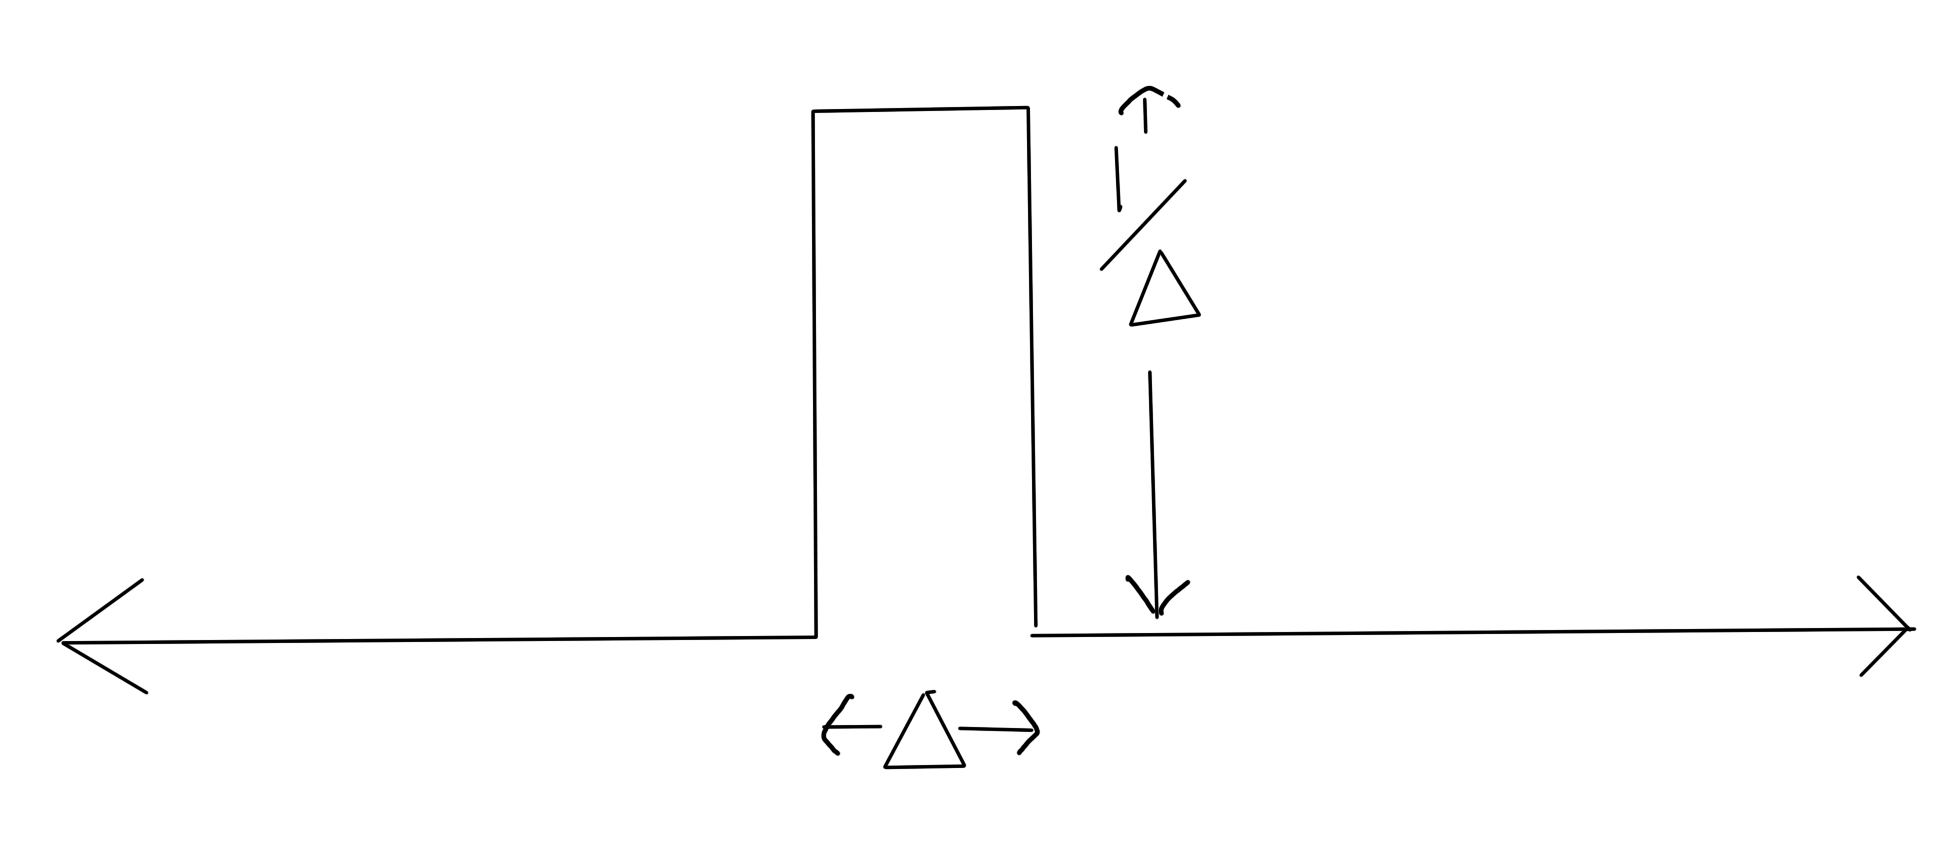
\includegraphics[width=0.5\textwidth]{delta1.png}
	\caption{The $\delta_\Delta$ function, centred at the origin}
\end{figure}
Thus, the area under the function, i.e. the integral of the function from $-\infty$ to $+\infty$ is unity, while the function is zero at all points except the origin.\\
\indent It should be noted that the delta function is not a function in the conventional sense. This is because, the delta function does not have a well-defined value at the origin. We call the delta function a ``generalized function". Generalized functions are generalizations or extensions of the concept of a function, but are not really functions.\\
\indent We will also refer to the delta function as a ``unit impulse". The unit impulse captures an area of unity while having zero width. The conventional way of representing a unit impulse is shown in fig. 2.\\
\begin{figure}[H]
	\centering
	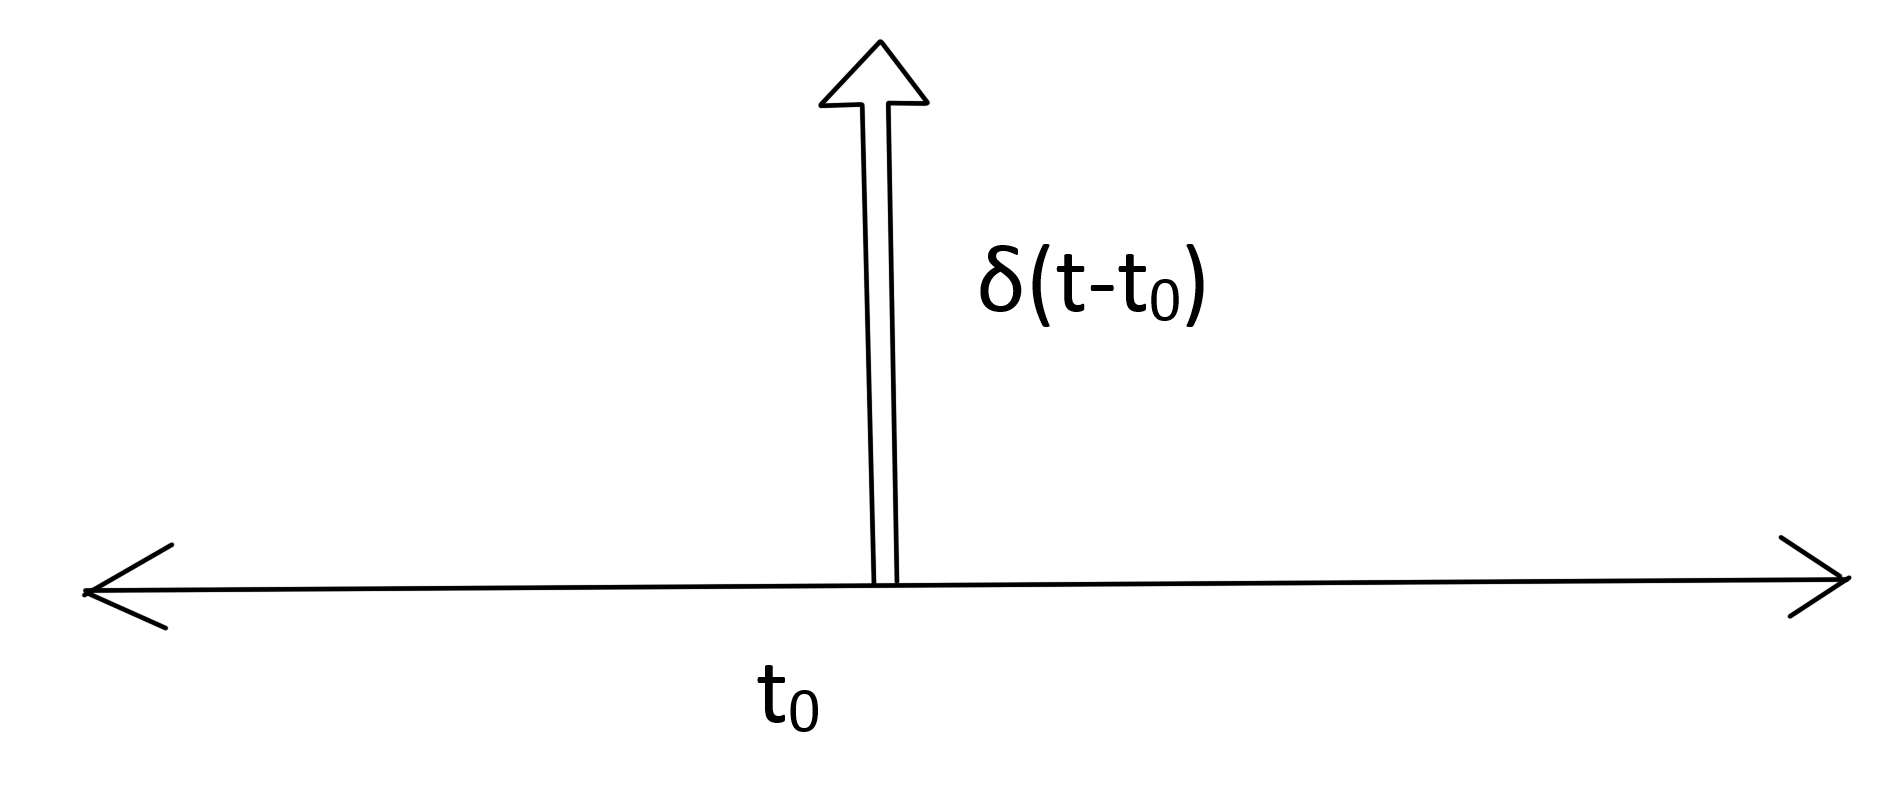
\includegraphics[width=0.5\textwidth]{delta2.png}
	\caption{Representing the unit impulse graphically}
\end{figure}
\indent Now, if we use the symbol $\delta_\Delta (t)$ for the above mentioned function with finite $\Delta$, then in accordance with the definition above,
$$\lim_{\Delta\rightarrow 0}\delta_\Delta(t)=\delta(t)$$
Where, we denote by $\delta(t)$ the unit impulse function.
%\subsection{Using unit impulse to get the value of a function at a particular point}
%We can get back the value of a function at a particular point if we integrate the delta function weighted properly, as is in the following equation:
%$$x(t_0)=\int_{-\infty}^{\infty	} x(t)\delta(t_0-t)dt$$
%\indent Thus, the delta function centred at a particular point multiplied by a function, gives the value of the function at that point when integrated over the entire real axis.

\subsection{Unit Impulse Response}
Assume that we give to a system, a unit impulse/delta function as its input. The output that is obtained is called the impulse response of that system. \\
\indent Although practically, we cannot generate an impulse function, one can imagine giving to the system $\delta_\Delta$ functions as inputs, successively, with decreasing values of $\Delta$ and obtain a good estimate of the Unit Impulse Response.\\
\indent Thus, in short, \textbf{the impulse response is the output of a system, when the input is a unit impulse.} (Fig. 3)
\begin{figure}[H]
	\centering
	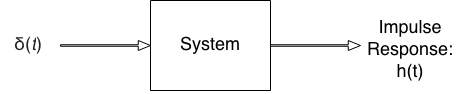
\includegraphics[width=0.5\textwidth]{Block-impulseresponse.png}
	\caption{Unit Impulse Response}
\end{figure}

\subsubsection{Impulse response of an LSI system}
Consider a linear shift-invariant system \textbf{S}. Now, suppose that we give as the input, the sum of two unit impulses centred at two different points $t_1$ and $t_2$. Due to additivity, we expect the output to be the sums of the corresponding outputs. (fig. 4(a))\\
\indent Also, because of homogeneity, we expect that the output corresponding to the input $\kappa\delta(t)$ should be $\kappa h(t)$ where h(t) is the unit impulse response and $\kappa\in\mathbb{C}$ (fig. 4(b))
\begin{figure}[H]
    \centering
    
\includegraphics[width=\textwidth]{Block-additivityimpulseresponse1}
    \caption{Consequence of Additivity of \textbf{S}}
\end{figure}
\begin{figure}[H]
	\centering
    % 
\includegraphics[width=\textwidth]{block-homogeneity}
    \begin{tikzpicture}

\node[coordinate]       (c0) {};	
\node[coordinate,label =above:{$k\delta[t]$},right=of c0](c1){};	
\node[dspfilter,right= of c1,text height=3em,text width=8em,text depth=3em]                    (c2) { System };
\node[coordinate,label=above:{$kh[t]$},right=of c2]             (c3) {};
\node[coordinate,right=of c3]          (c4) {};
		
\foreach \i [evaluate = \i as \j using int(\i+2)] in {0,2}
\draw[dspconn] (c\i) -- (c\j);

\end{tikzpicture}
    \caption{Consequence of Homogeneity of \textbf{S}}
\end{figure}

Now, if we took $\kappa$ to be the value of a function $x$ at some point, then the property still holds.\\
\indent Let us not consider the output of $\delta(t-t_0)$, which is nothing but $\delta(t)$ shifted to the right by $t_0$ units. Thus, due to shift invariance, we expect that the output to $\delta(t-t_0)$ should be $h(t-t_0)$.(fig. 5)

\begin{figure}[H]
	\centering
	
\includegraphics[width=0.7\textwidth]{Block-shiftinv.png}
	\caption{Consequence of shift-invariance of \textbf{S}}
\end{figure}

Now assume that we have points $\lambda_1$, $\lambda_2$ and $\lambda_3$. As a consequence of Homogeneity, Additivity and Shift-Invariance of \textbf{S}, we know that the output corresponding to $x(\lambda_1)\delta(t-\lambda_1)+x(\lambda_2)\delta(t-\lambda_2)+x(\lambda_3)\delta(t-\lambda_3)$ will be $x(\lambda_1)h(t-\lambda_1)+x(\lambda_2)h(t-\lambda_2)+x(\lambda_3)h(t-\lambda_3)$.\\
\indent We can think of an integral as a summation of many such products $x(\lambda)\delta(t-\lambda)$ where the $\lambda$'s are brought infinitesimally close to each other. Thus, we can consider the integration as a summation over a continuum of $\lambda$'s. (fig. 6)

\begin{figure}[H]
	\centering
	
\includegraphics[width=0.8\textwidth]{Block-characterization1.png}
	\caption{Consequence of Linear shift-invariance of \textbf{S}}
\end{figure}
\indent As discussed in the previous lecture, the input integral equates to $x(t)$. Thus, we have obtained a way of obtaining the output corresponding to any signal $x(t)$ using the impulse response.\\\\
\noindent\fbox{%
    \parbox{\textwidth}{%
       \textbf{Given the impulse response of an Linear Shift-Invariant System, we can calculate the output corresponding to any input signal.}
    }%
}
\\\\
This is a very important result in signals and systems, because knowing the output of just one function gives us the power to know beforehand, what the output should be for any input provided to the LSI system.
